% !TEX encoding = UTF-8 Unicode
\documentclass[12pt, A4,onecolumn]{article} %se puede poner twocolumn
\usepackage[normalem]{ulem} %tachar
\usepackage{cite}
\usepackage[utf8]{inputenc}
\usepackage{verbatim} %para comentarios 
%\usepackage[spanish]{babel}
\usepackage[hidelinks]{hyperref} %para que no salga en rojo
\usepackage{color} %para poder escribir con colores
\usepackage[margin=2.5cm]{geometry} %para modificar margenes
\usepackage{listings} %para insertar código
\usepackage[table,xcdraw]{xcolor} %para insertar tablas con color
\usepackage{amsmath} %para matrices
\usepackage{graphicx} %para insertar imagenes
\usepackage{float}
\usepackage{subcaption} % loads the caption package
\usepackage{multirow}
\definecolor{dkgreen}{rgb}{0,0.6,0}
\definecolor{gray}{rgb}{0.5,0.5,0.5}
\definecolor{mauve}{rgb}{0.58,0,0.82}
\graphicspath{ {Machintosh_HD/Utenti/admin/Scrivania} }


\title{\textbf{Machine Learning\\ 
\small{by Stanford University}\\
Week1
}}
\author{
Jose Vicente Yago Martínez
}%\date{28/3/2019}


\begin{document}
\maketitle

	
%\vfill
%\centering
%\textit{Lecturer:} \\
%AndrewNg


%\begin{figure}[H]
%	\centering
%	\includegraphics[width=0.2\textwidth]{logo-fium}
%\end{figure}	



\newpage
\tableofcontents
%\listoffigures

\newpage

% -----------------------------------------------------------------------------------%
% -----------------------------------------------------------------------------------%
%------------------------------------INTRO---------------------------------------%
% -----------------------------------------------------------------------------------%
% -----------------------------------------------------------------------------------%
\section{Introduction}
\subsection{What is machine learning?}
Two definitions of Machine Learning are offered. Arthur Samuel described it as: "the field of study that gives computers the ability to learn without being explicitly programmed." This is an older, informal definition.

Tom Mitchell provides a more modern definition: "A computer program is said to learn from experience E with respect to some class of tasks T and performance measure P, if its performance at tasks in T, as measured by P, improves with experience E."



Example: playing checkers.

E = the experience of playing many games of checkers

T = the task of playing checkers.

P = the probability that the program will win the next game.

In general, any machine learning problem can be assigned to one of two broad classifications:

Supervised learning and Unsupervised learning.

\subsection{Supervised learning}
In supervised learning, we are given a data set and already know what our correct output should look like, having the idea that there is a relationship between the input and the output.

Supervised learning problems are categorized into "regression" and "classification" problems. In a regression problem, we are trying to predict results within a continuous output, meaning that we are trying to map input variables to some continuous function. In a classification problem, we are instead trying to predict results in a discrete output. In other words, we are trying to map input variables into discrete categories.
\\\\
\textbf{Example 1:}

Given data about the size of houses on the real estate market, try to predict their price. Price as a function of size is a continuous output, so this is a regression problem.

We could turn this example into a classification problem by instead making our output about whether the house "sells for more or less than the asking price." Here we are classifying the houses based on price into two discrete categories.
\\\\
\textbf{Example 2:}

(a) Regression - Given a picture of a person, we have to predict their age on the basis of the given picture

(b) Classification - Given a patient with a tumor, we have to predict whether the tumor is malignant or benign.


\subsection{Unsupervised learning}
Unsupervised learning allows us to approach problems with little or no idea what our results should look like. We can derive structure from data where we don't necessarily know the effect of the variables.

We can derive this structure by clustering the data based on relationships among the variables in the data.

With unsupervised learning there is no feedback based on the prediction results.
\\\\
\textbf{Example:}

Clustering: Take a collection of 1,000,000 different genes, and find a way to automatically group these genes into groups that are somehow similar or related by different variables, such as lifespan, location, roles, and so on.

Non-clustering: The "Cocktail Party Algorithm", allows you to find structure in a chaotic environment. 


% -----------------------------------------------------------------------------------%
% -----------------------------------------------------------------------------------%
%--------------------------MODEL & COST FUNC--------------------------%
% -----------------------------------------------------------------------------------%
% -----------------------------------------------------------------------------------%
\section{Model and cost function}
\subsection{Model representation}
\begin{figure}[H]
	\centering
	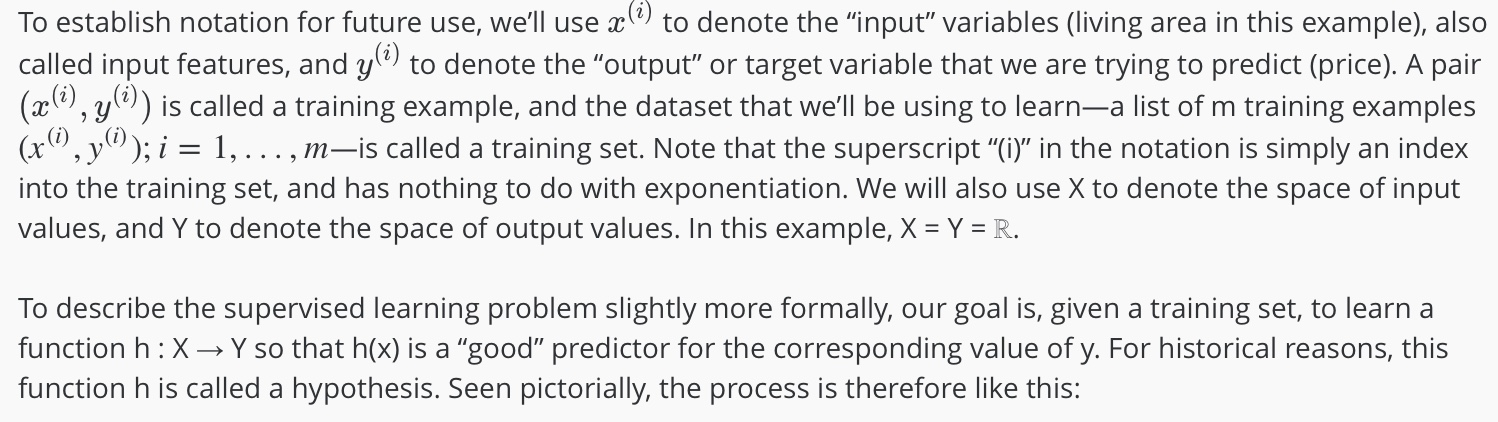
\includegraphics[width=1\textwidth]{./Imagenes/modelCost1}
\end{figure}	

\begin{figure}[H]
	\centering
	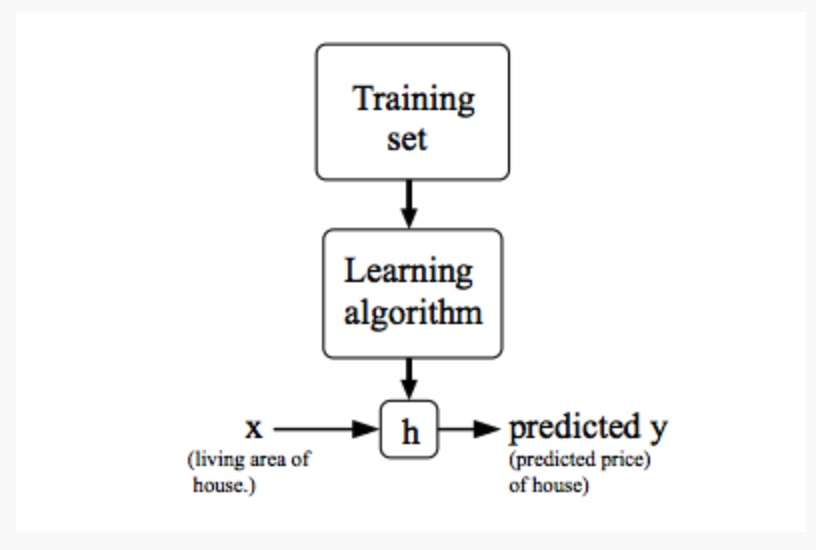
\includegraphics[width=0.5\textwidth]{./Imagenes/modelCost2}
\end{figure}	
When the target variable that we’re trying to predict is continuous, such as in our housing example, we call the learning problem a regression problem. When y can take on only a small number of discrete values (such as if, given the living area, we wanted to predict if a dwelling is a house or an apartment, say), we call it a classification problem.

\subsection{Cost function}
\subsubsection{Intuition I}
\begin{figure}[H]
	\centering
	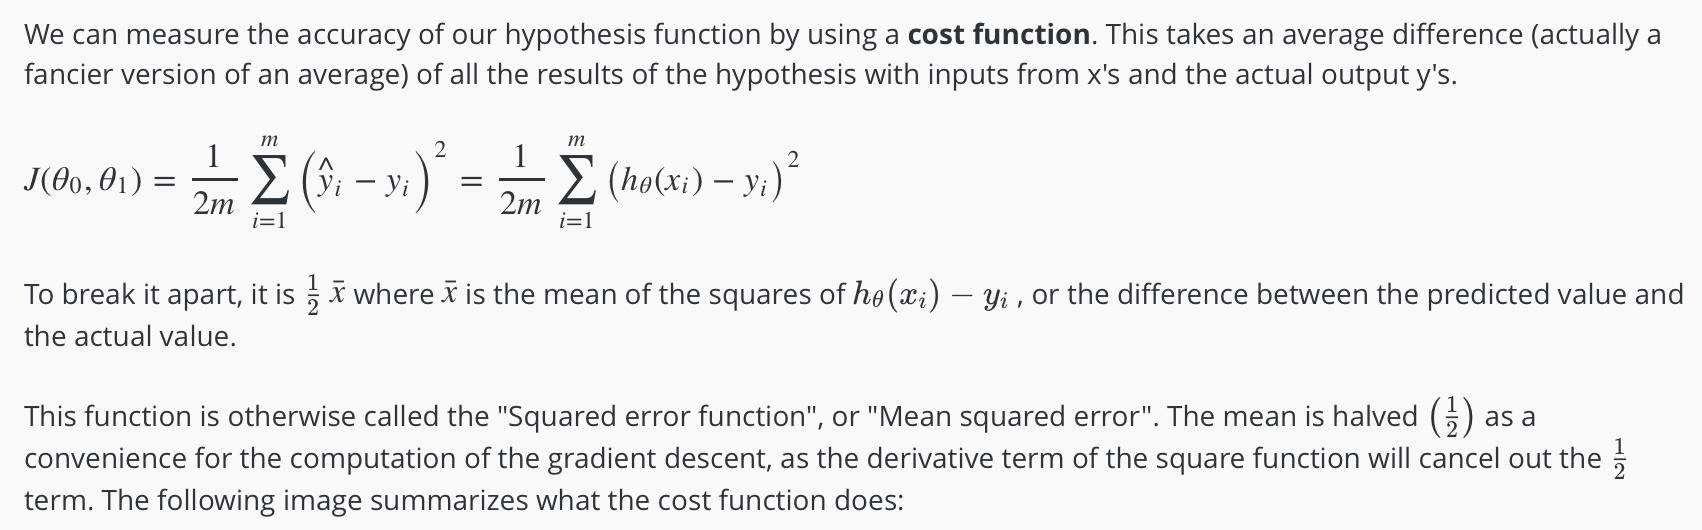
\includegraphics[width=1\textwidth]{./Imagenes/costFunc1}
\end{figure}	

\begin{figure}[H]
	\centering
	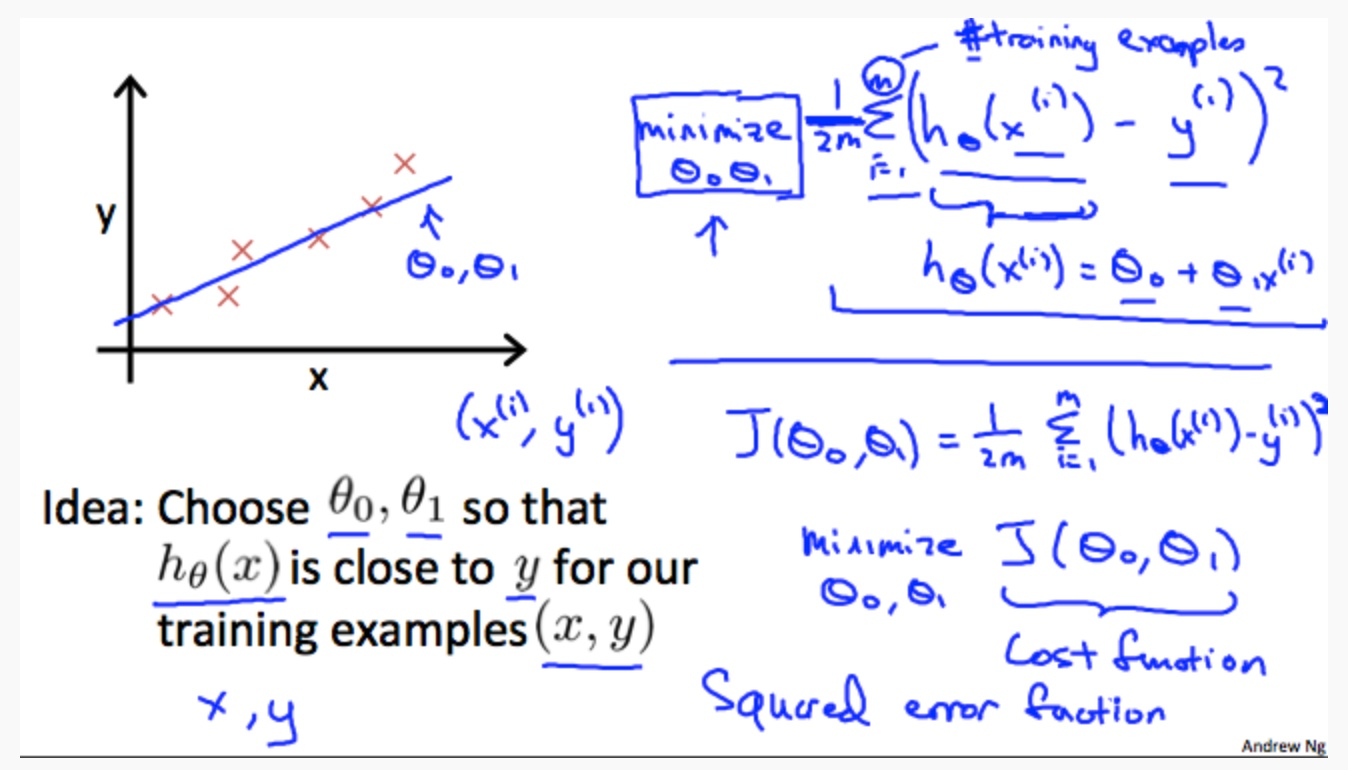
\includegraphics[width=0.8\textwidth]{./Imagenes/costFunc2}
\end{figure}	

\begin{figure}[H]
	\centering
	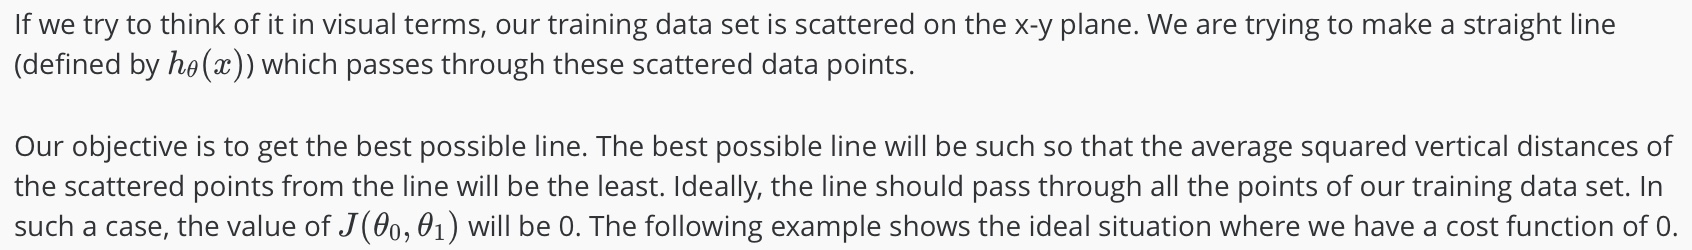
\includegraphics[width=1\textwidth]{./Imagenes/costFunc3}
\end{figure}	

\begin{figure}[H]
	\centering
	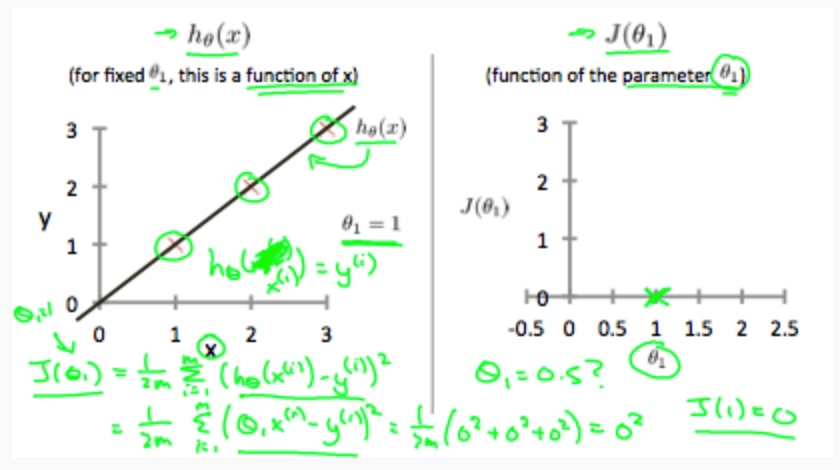
\includegraphics[width=0.8\textwidth]{./Imagenes/costFunc4}
\end{figure}	

\begin{figure}[H]
	\centering
	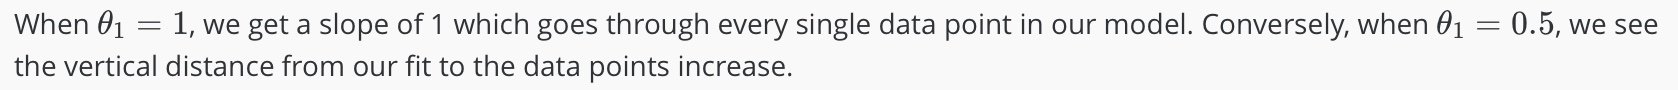
\includegraphics[width=1\textwidth]{./Imagenes/costFunc5}
\end{figure}	

\begin{figure}[H]
	\centering
	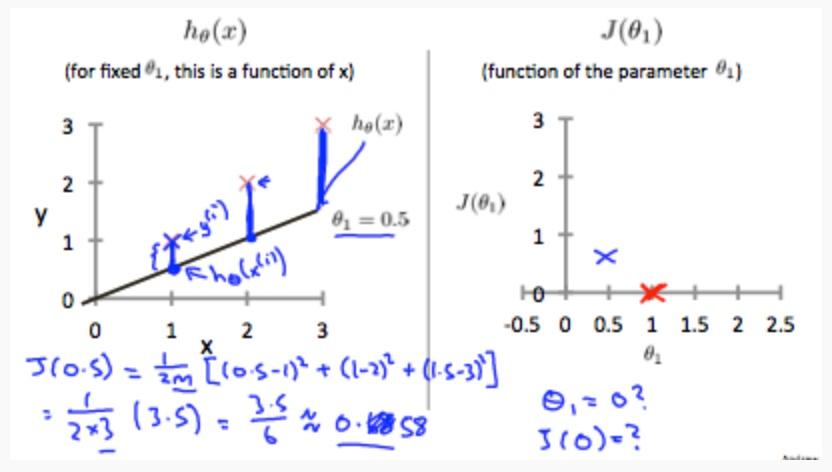
\includegraphics[width=0.8\textwidth]{./Imagenes/costFunc6}
\end{figure}	

This increases our cost function to 0.58. Plotting several other points yields to the following graph:

\begin{figure}[H]
	\centering
	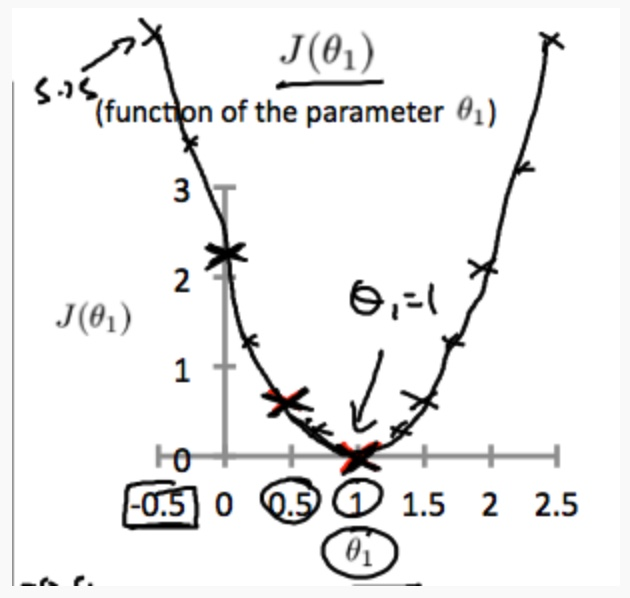
\includegraphics[width=0.5\textwidth]{./Imagenes/costFunc7}
\end{figure}	

\begin{figure}[H]
	\centering
	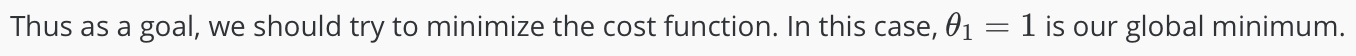
\includegraphics[width=1\textwidth]{./Imagenes/costFunc8}
\end{figure}	

\subsubsection{Intuition II}

\begin{figure}[H]
	\centering
	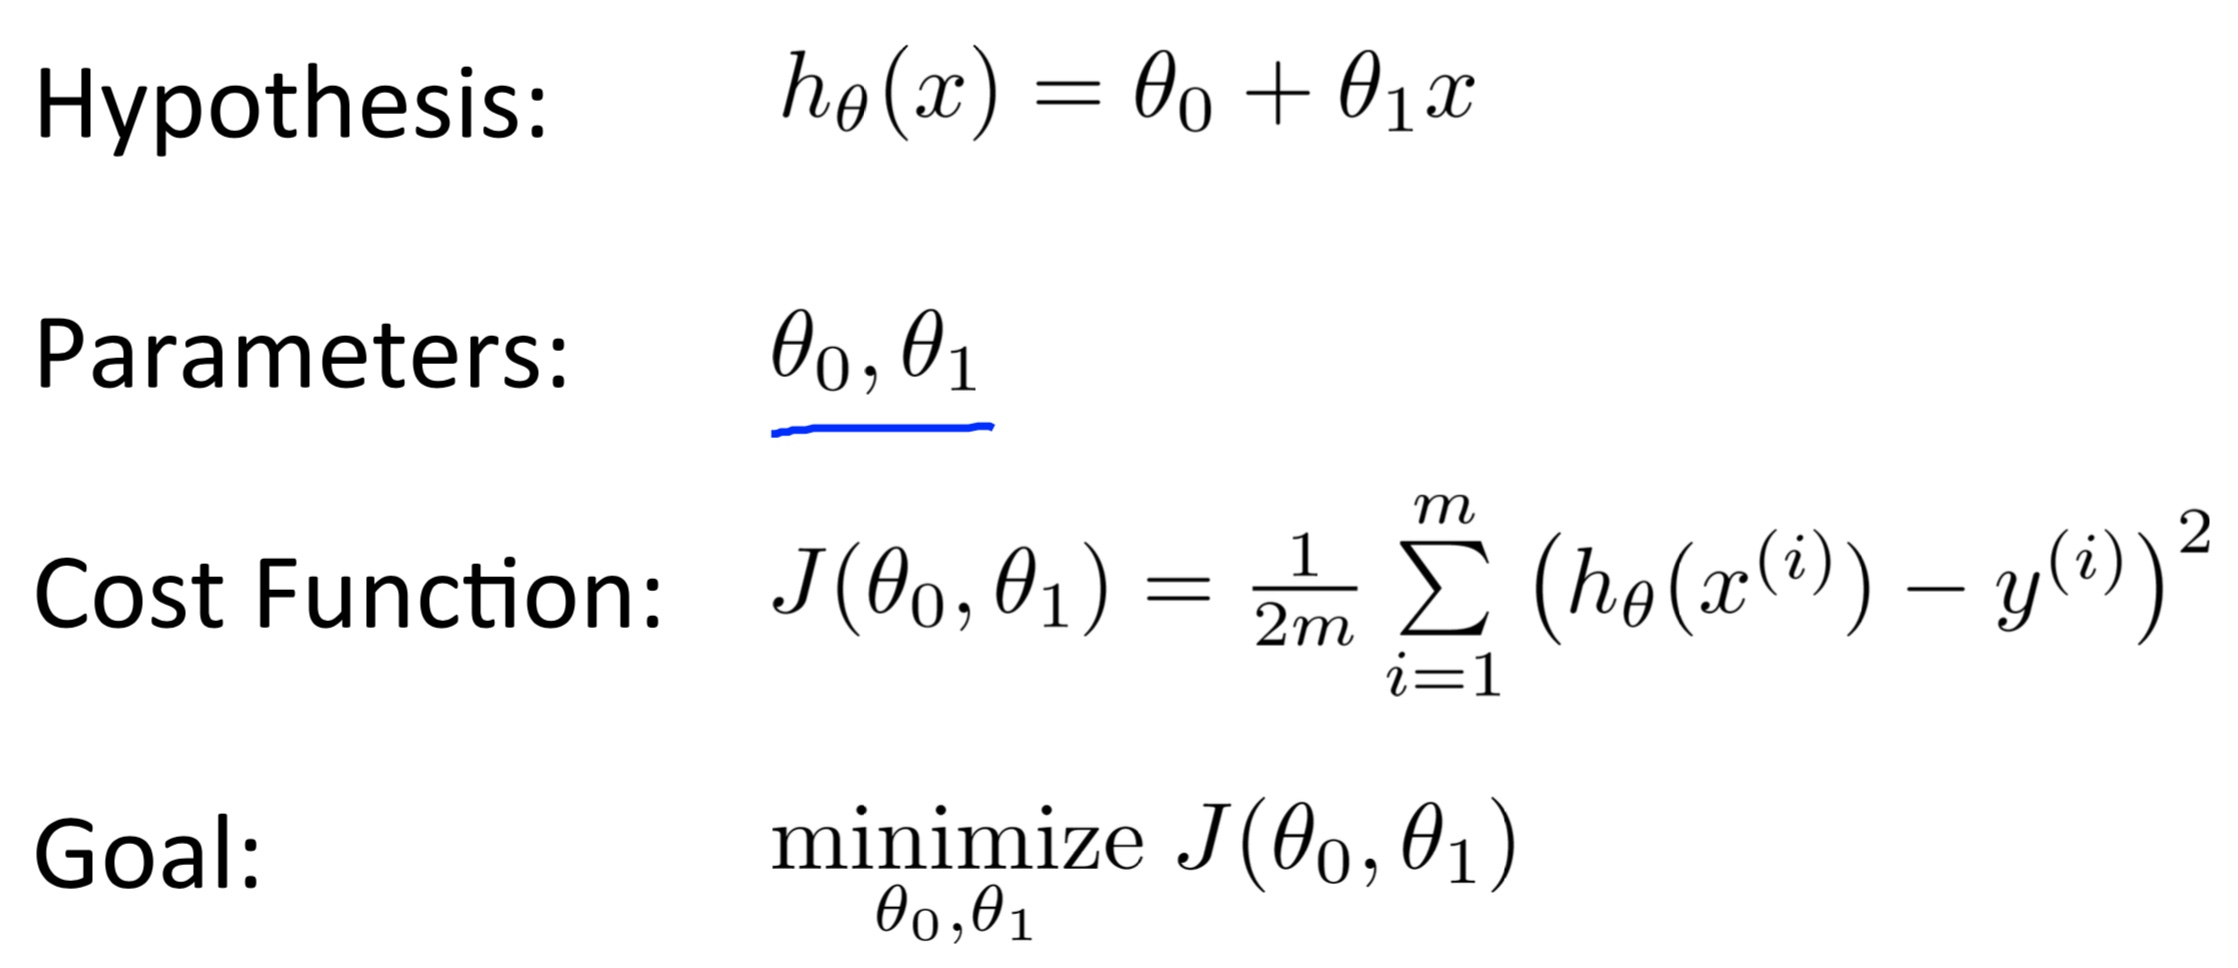
\includegraphics[width=0.8\textwidth]{./Imagenes/intuitionII}
\end{figure}	

A contour plot is a graph that contains many contour lines. A contour line of a two variable function has a constant value at all points of the same line. An example of such a graph is the one to the right below.
\begin{figure}[H]
	\centering
	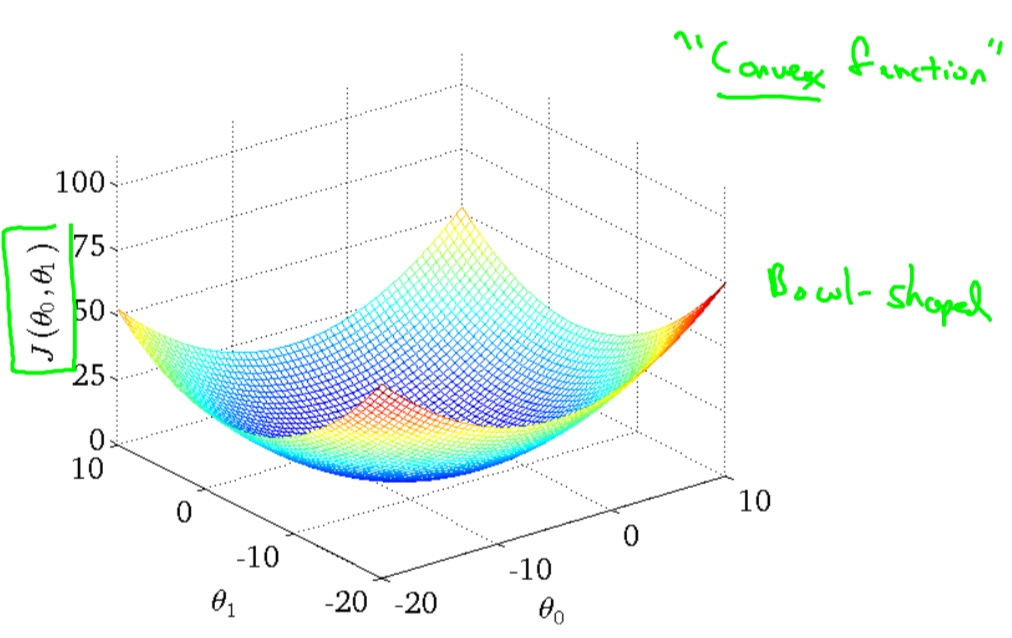
\includegraphics[width=0.9\textwidth]{./Imagenes/convexFunc}
\end{figure}	

\begin{figure}[H]
	\centering
	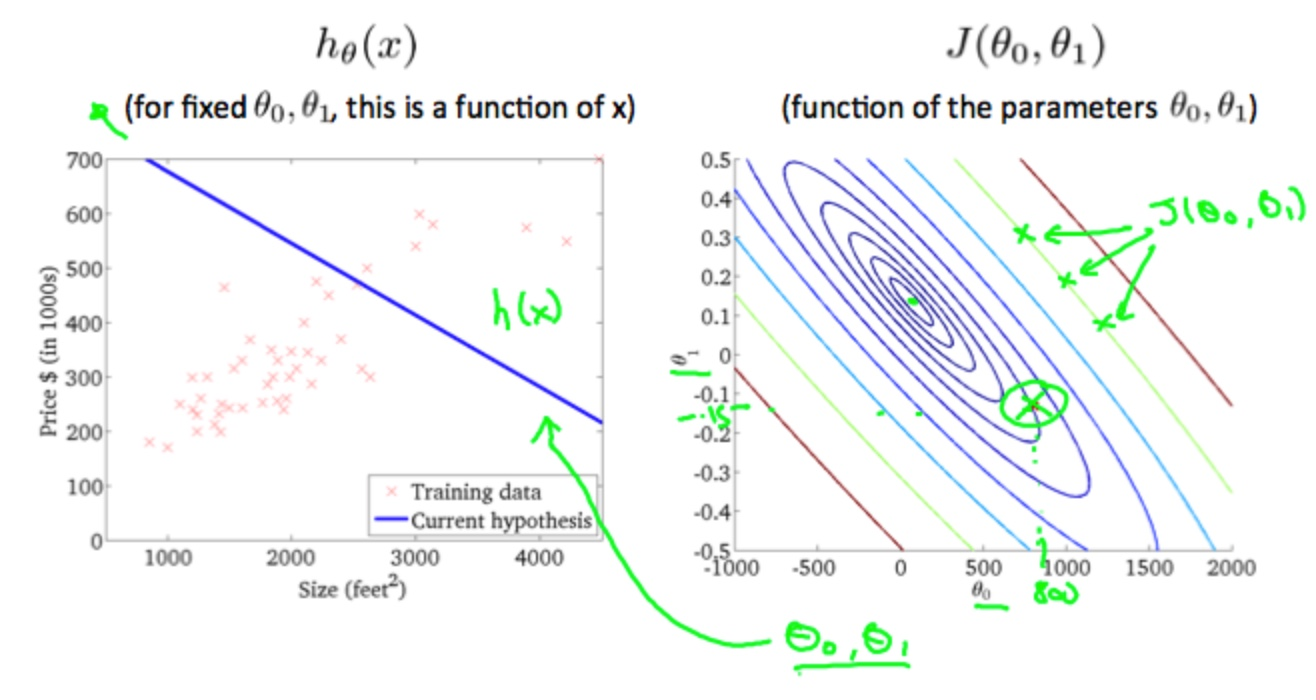
\includegraphics[width=1\textwidth]{./Imagenes/costFunc9}
\end{figure}	

\begin{figure}[H]
	\centering
	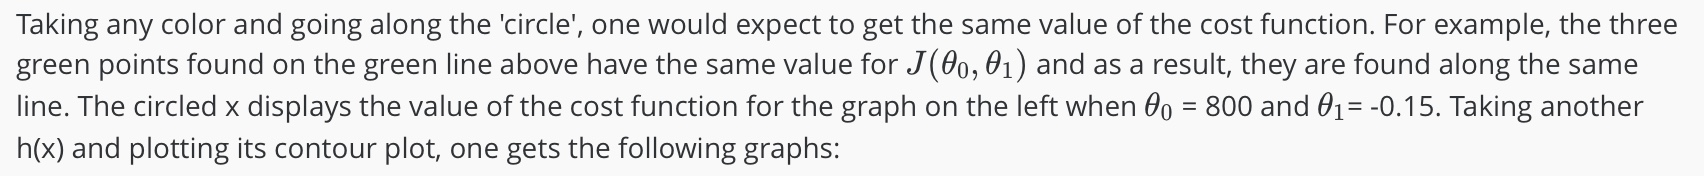
\includegraphics[width=1\textwidth]{./Imagenes/costFunc10}
\end{figure}	

\begin{figure}[H]
	\centering
	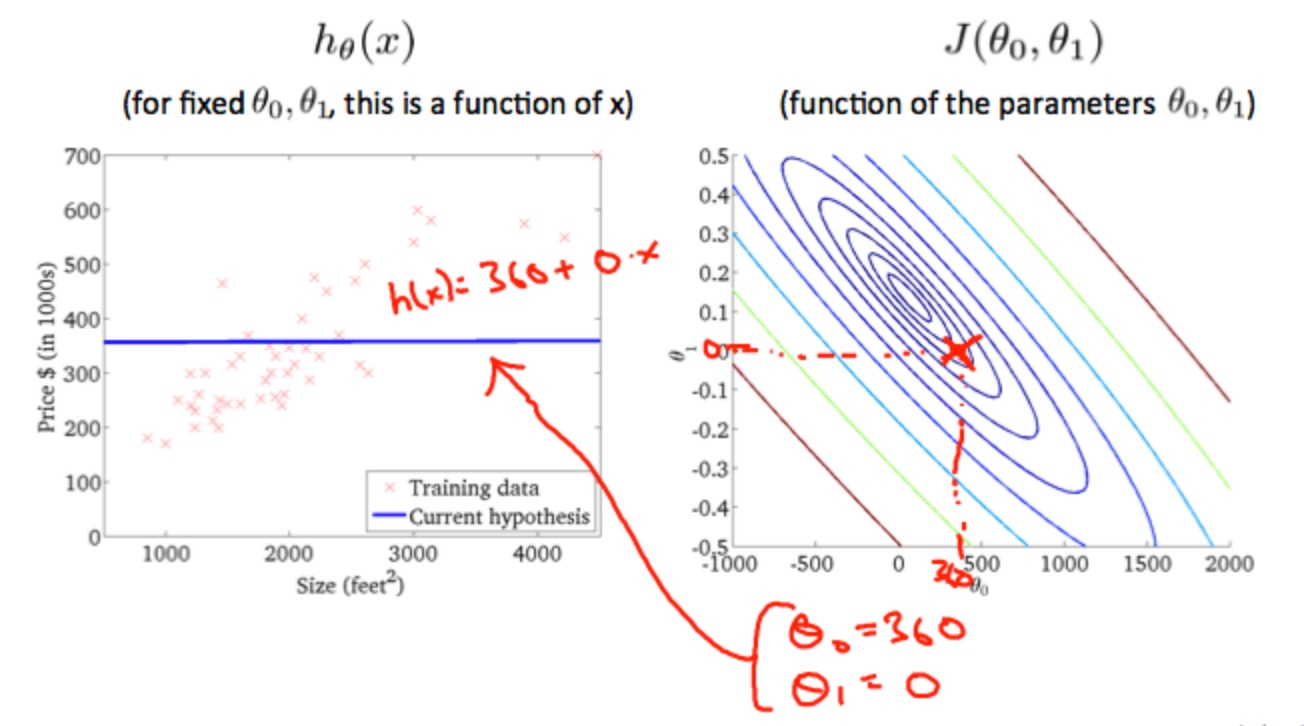
\includegraphics[width=1\textwidth]{./Imagenes/costFunc11}
\end{figure}	

\begin{figure}[H]
	\centering
	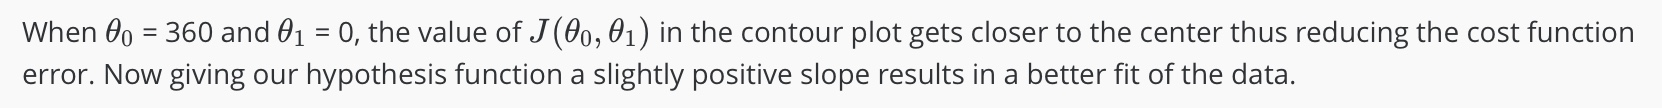
\includegraphics[width=1\textwidth]{./Imagenes/costFunc12}
\end{figure}

\begin{figure}[H]
	\centering
	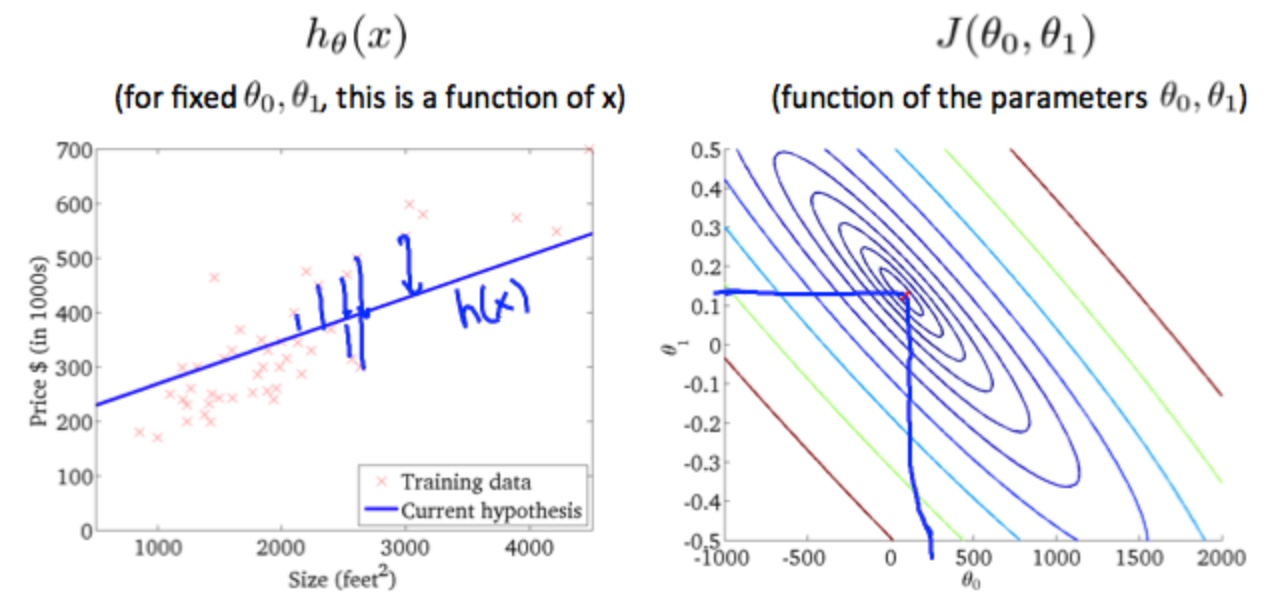
\includegraphics[width=1\textwidth]{./Imagenes/costFunc13}
\end{figure}

\begin{figure}[H]
	\centering
	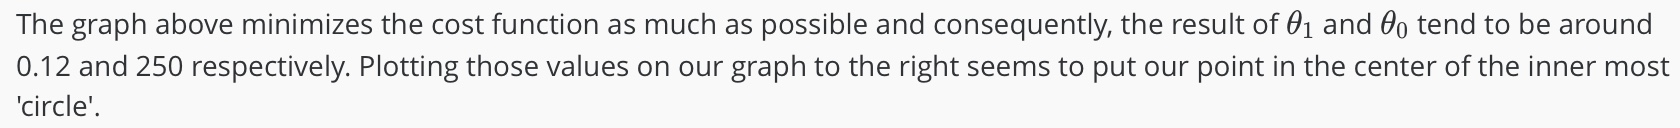
\includegraphics[width=1\textwidth]{./Imagenes/costFunc14}
\end{figure}

% -----------------------------------------------------------------------------------%
% -----------------------------------------------------------------------------------%
%-----------------------PARAMETER LEARNING--------------------------%
% -----------------------------------------------------------------------------------%
% -----------------------------------------------------------------------------------%
\section{Parameter learning}

\subsection{Gradient descent intuition}
\begin{figure}[H]
	\centering
	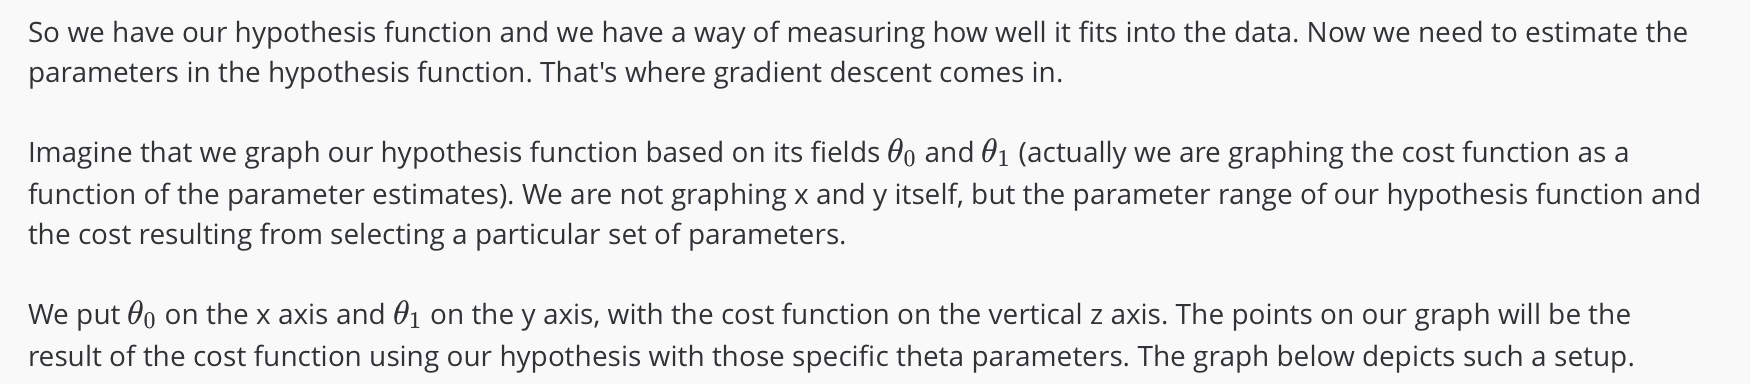
\includegraphics[width=1\textwidth]{./Imagenes/gradient1}
\end{figure}

\begin{figure}[H]
	\centering
	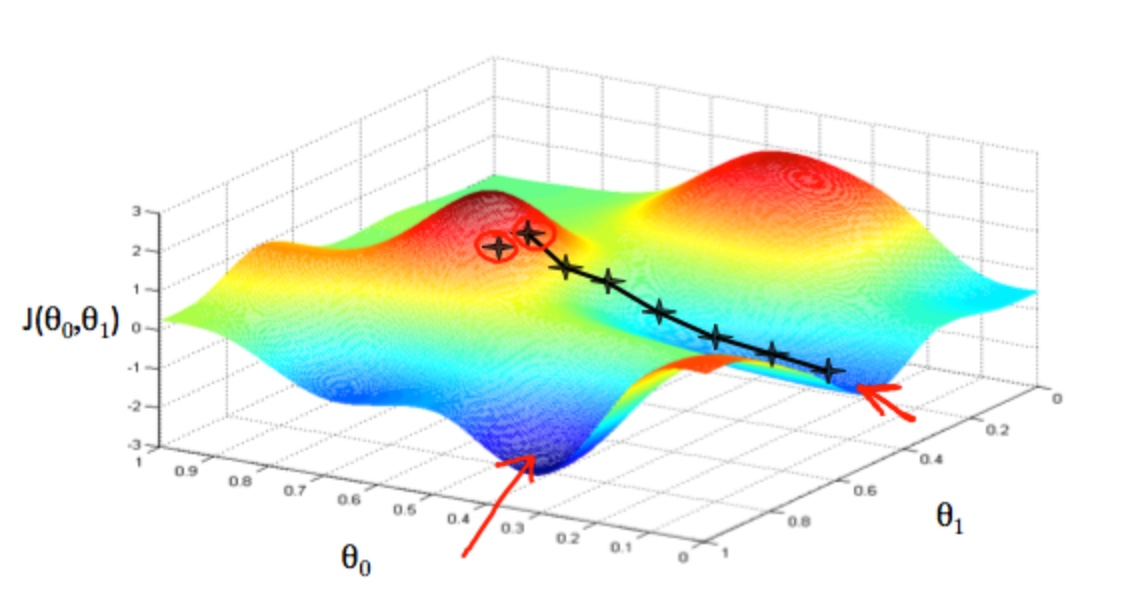
\includegraphics[width=1\textwidth]{./Imagenes/gradient2}
\end{figure}

\begin{figure}[H]
	\centering
	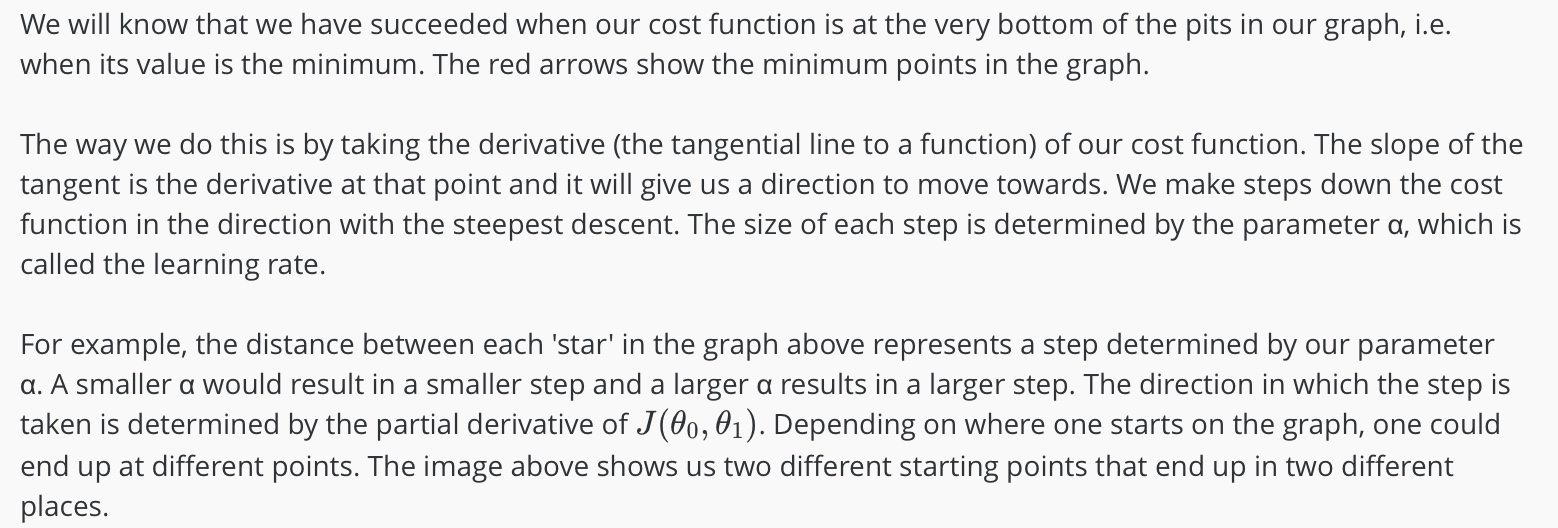
\includegraphics[width=1\textwidth]{./Imagenes/gradient3}
\end{figure}

\begin{figure}[H]
	\centering
	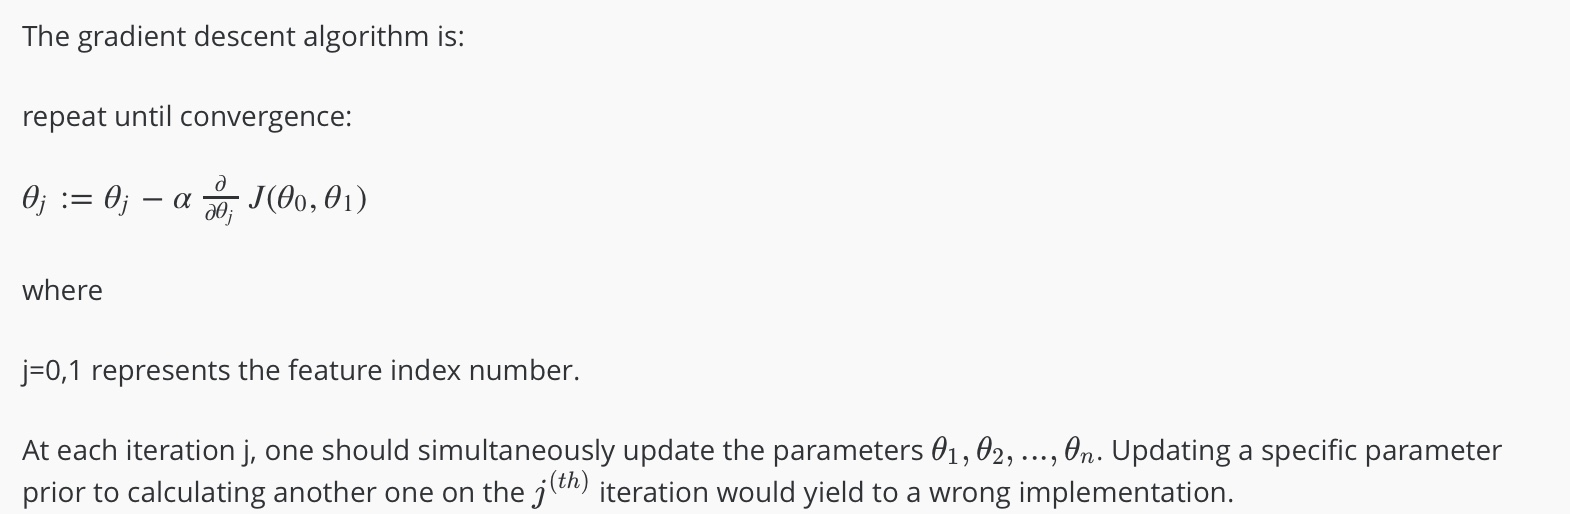
\includegraphics[width=1\textwidth]{./Imagenes/gradient4}
\end{figure}

\begin{figure}[H]
	\centering
	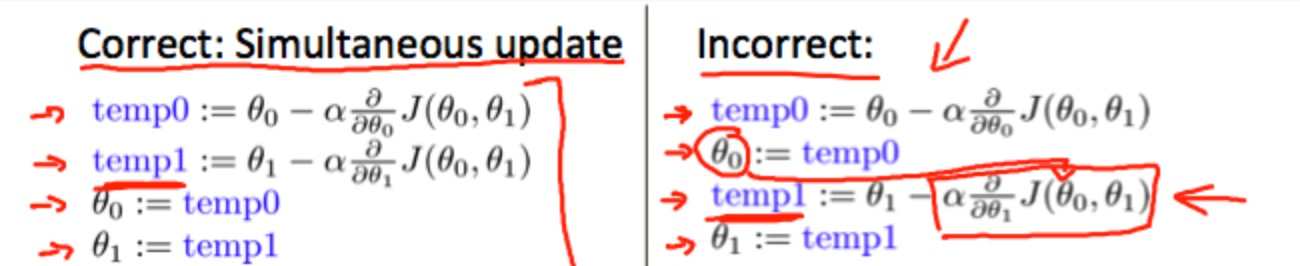
\includegraphics[width=1\textwidth]{./Imagenes/gradient5}
\end{figure}

\begin{figure}[H]
	\centering
	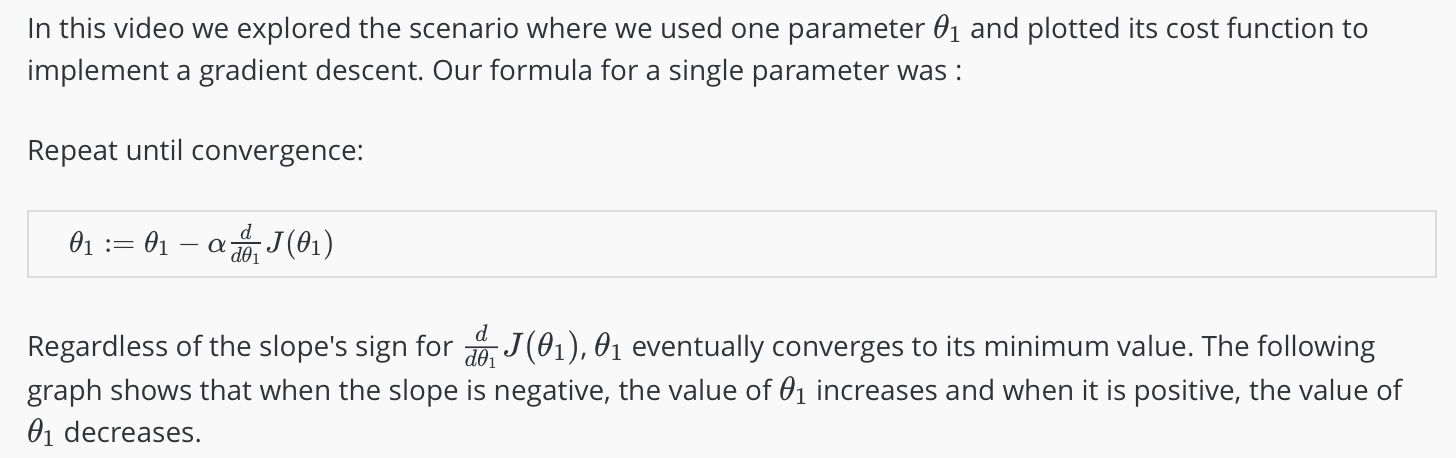
\includegraphics[width=1\textwidth]{./Imagenes/gradient6}
\end{figure}

\begin{figure}[H]
	\centering
	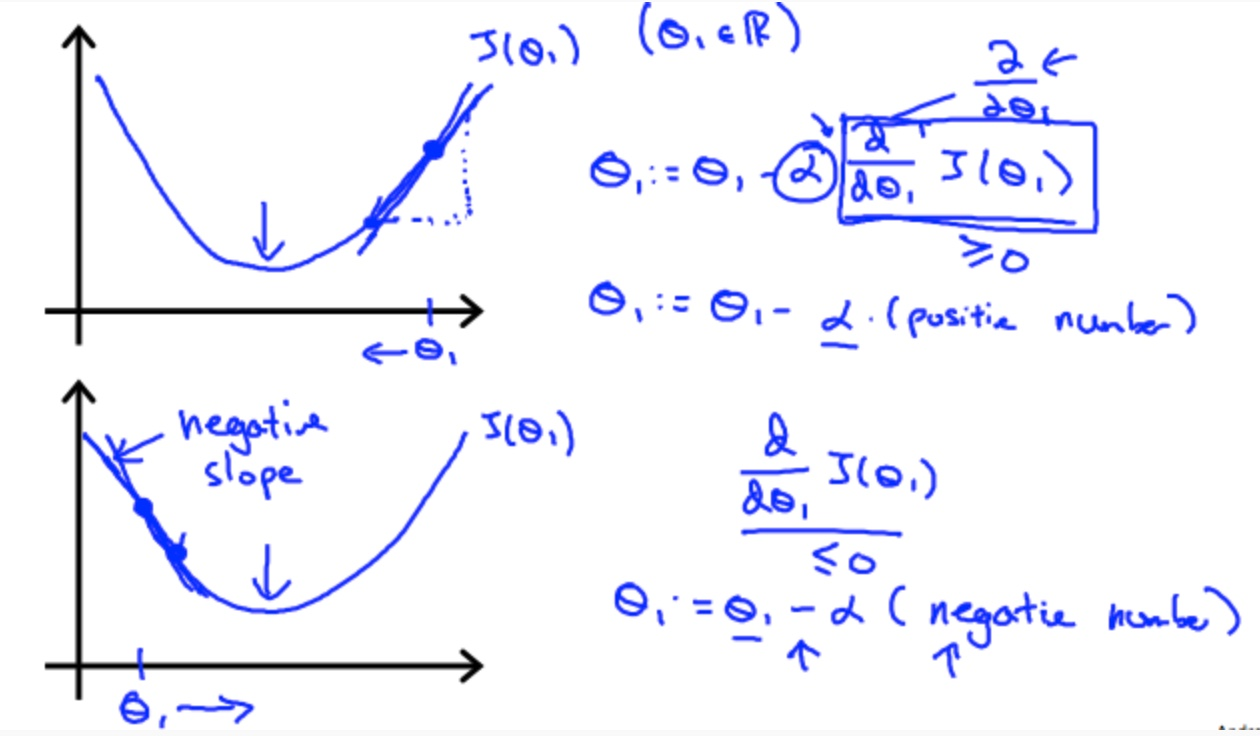
\includegraphics[width=1\textwidth]{./Imagenes/gradient7}
\end{figure}

\begin{figure}[H]
	\centering
	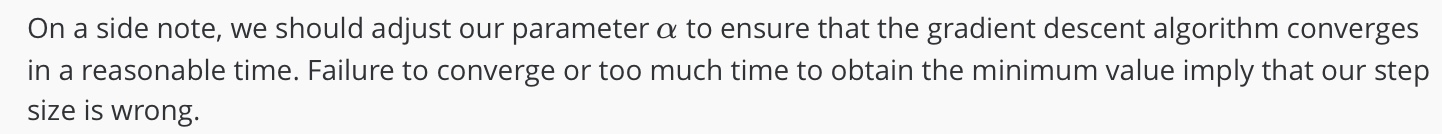
\includegraphics[width=1\textwidth]{./Imagenes/gradient8}
\end{figure}

\begin{figure}[H]
	\centering
	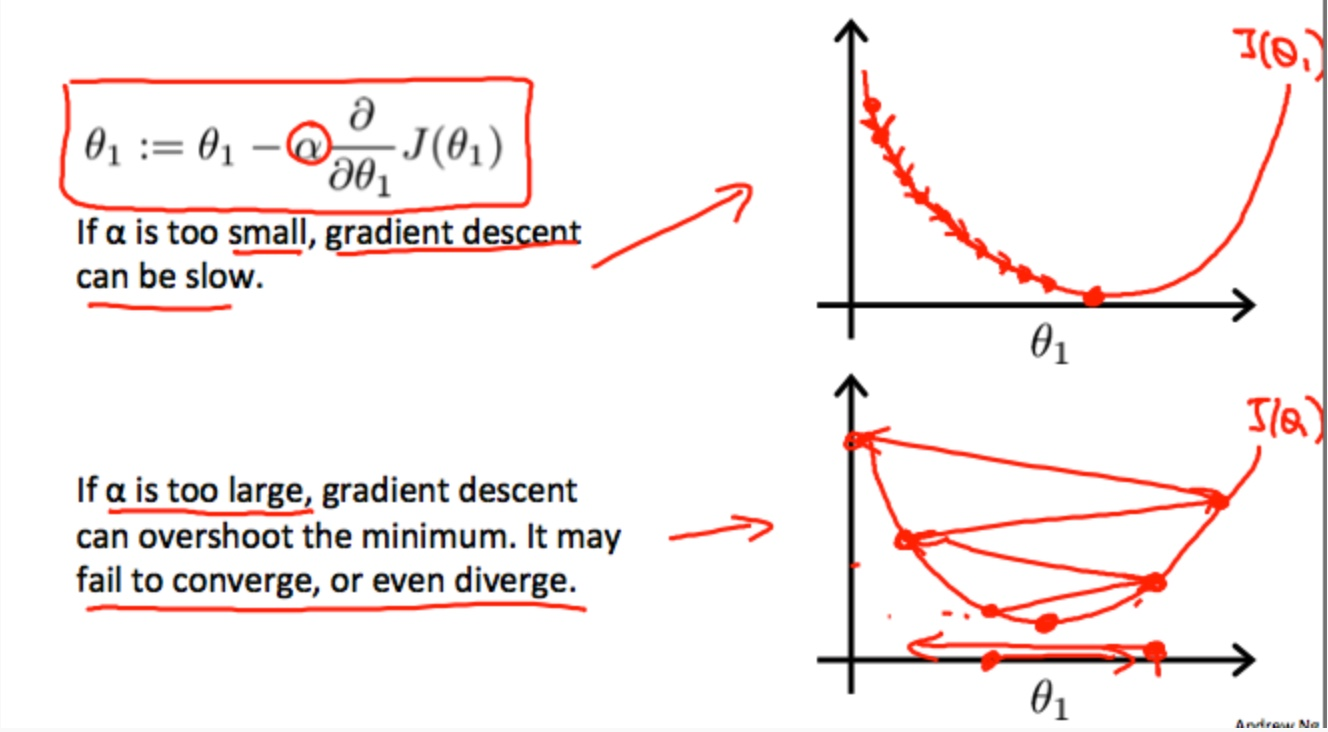
\includegraphics[width=1\textwidth]{./Imagenes/gradient9}
\end{figure}

\begin{figure}[H]
	\centering
	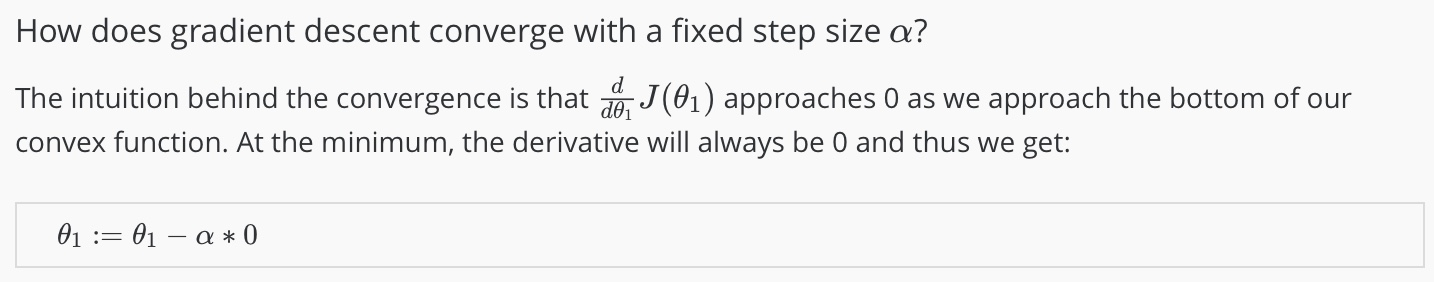
\includegraphics[width=1\textwidth]{./Imagenes/gradient10}
\end{figure}

\begin{figure}[H]
	\centering
	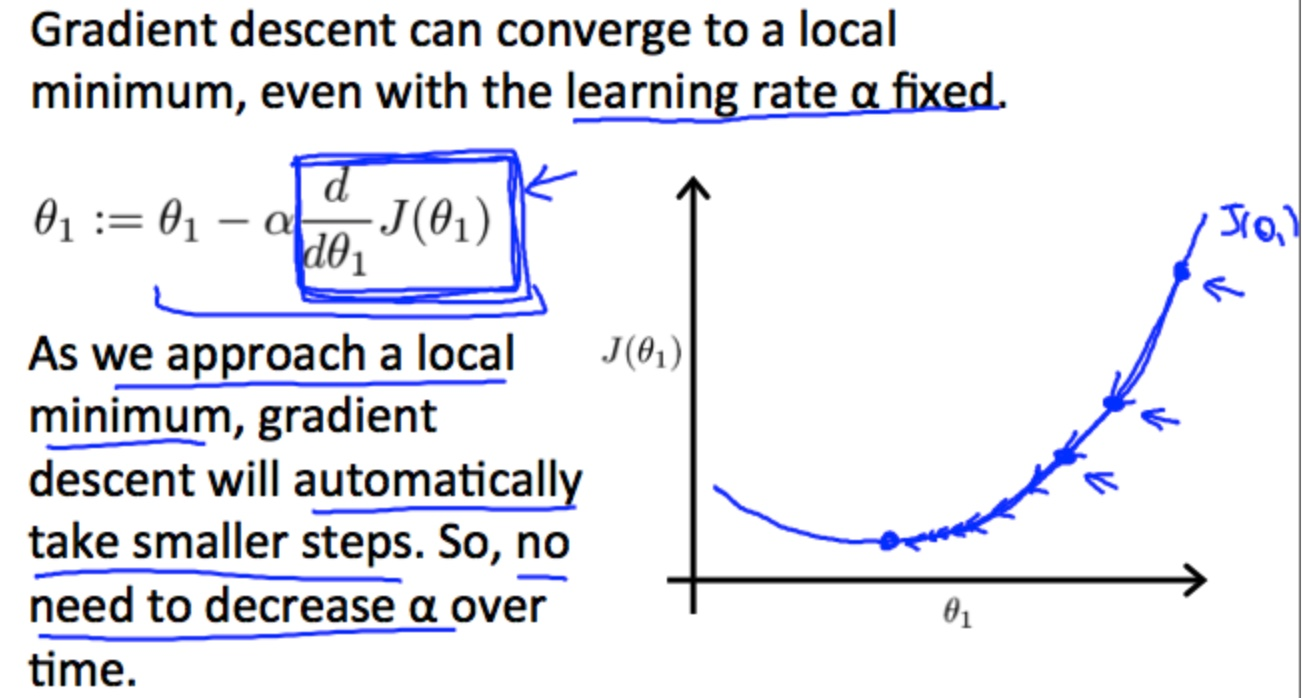
\includegraphics[width=1\textwidth]{./Imagenes/gradient11}
\end{figure}

\subsection{Gradient descent for linear regression}

When specifically applied to the case of linear regression, a new form of the gradient descent equation can be derived. We can substitute our actual cost function and our actual hypothesis function and modify the equation to :
\begin{figure}[H]
	\centering
	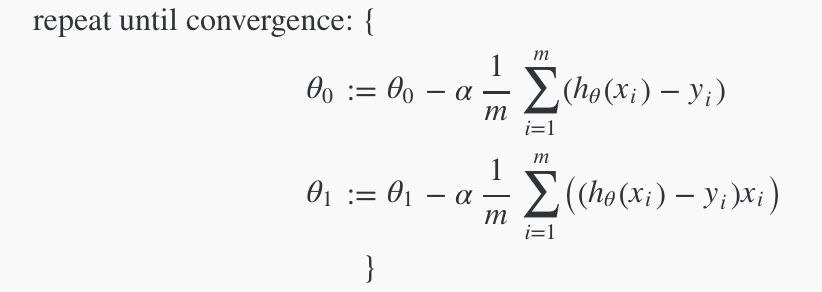
\includegraphics[width=1\textwidth]{./Imagenes/gradient12}
\end{figure}

\begin{figure}[H]
	\centering
	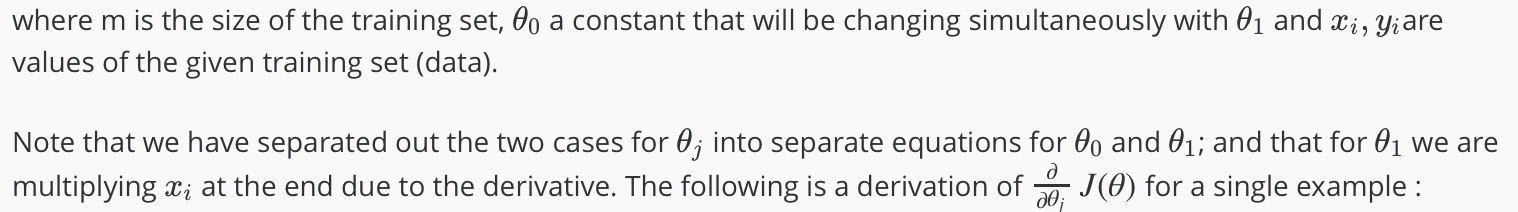
\includegraphics[width=1\textwidth]{./Imagenes/gradient13}
\end{figure}

\begin{figure}[H]
	\centering
	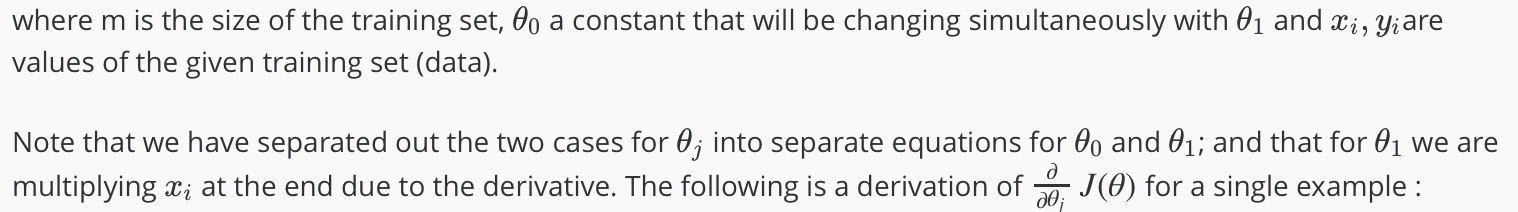
\includegraphics[width=1\textwidth]{./Imagenes/gradient13}
\end{figure}

\begin{figure}[H]
	\centering
	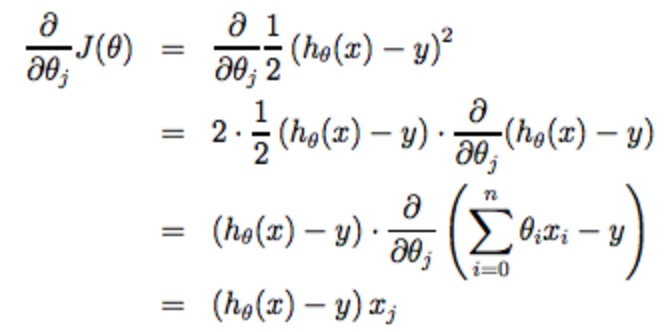
\includegraphics[width=0.6\textwidth]{./Imagenes/gradient14}
\end{figure}

\begin{figure}[H]
	\centering
	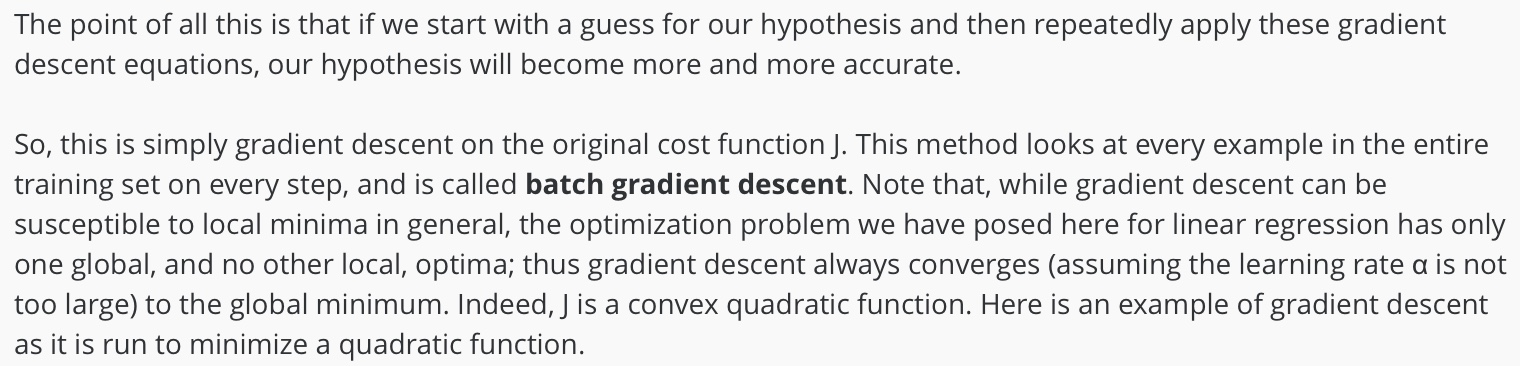
\includegraphics[width=1\textwidth]{./Imagenes/gradient15}
\end{figure}

\begin{figure}[H]
	\centering
	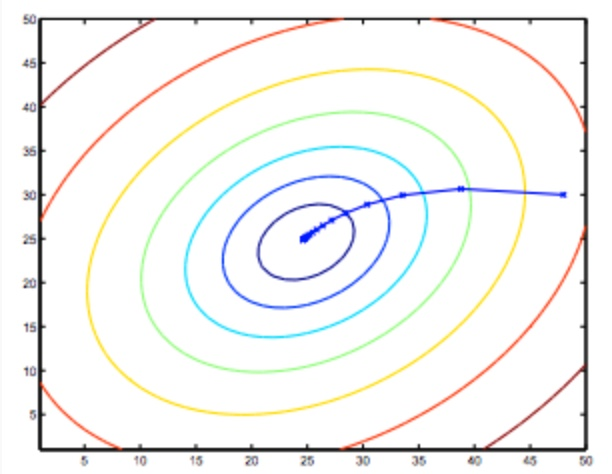
\includegraphics[width=0.45\textwidth]{./Imagenes/gradient16}
\end{figure}

\end{document}
